\documentclass[
	letterpaper, % Use US letter paper size
]{jdf}

\usepackage{todonotes}
\usepackage{fvextra}  % word-wrapping verbatim for chat transcripts
\DefineVerbatimEnvironment{transcript}{Verbatim}{breaklines, breakanywhere, fontsize=\small}
\addbibresource{references.bib}

\author{Your Name}
\email{youremail@gatech.edu}
\title{SAMI Assignment:\\Interaction Audit \& Redesign Challenge}

\begin{document}

\maketitle

% NOTE (delete before submission): The survey is part of this assignment.
% The rendered reminder below makes the link easy to find; delete it before
% you submit.
\begin{center}
	\textit{This assignment includes a survey — please complete it:}\\
	\href{https://gatech.co1.qualtrics.com/jfe/form/SV_9WAM09y6C74uKcm}{https://gatech.co1.qualtrics.com/jfe/form/SV\_9WAM09y6C74uKcm}\\
	\textit{Delete this notice before submitting.}
\end{center}

% =============================================================================
% ASSIGNMENT OVERVIEW (for your reference — not rendered in the PDF)
% =============================================================================
% THE GOAL: Imagine you are the Lead Developer for SAMI this semester. Your
% goal is to audit its current performance and draft a one-semester development
% roadmap to improve it with what you have learned in the KBAI class.
%
% SAMI is a social agent that uses a knowledge graph to model users and make
% matchmaking recommendations connecting students with one another.
%
% TWO PARTS:
%   Part 1 — The Interaction Audit: stress-test SAMI's current logic and
%     behavior, record your findings, and reflect on its performance.
%   Part 2 — The Redesign Challenge: propose a feasible one-semester
%     improvement plan as a concise "Product Roadmap."
%
% SURVEY: Please fill out the survey as part of the assignment:
%   https://gatech.co1.qualtrics.com/jfe/form/SV_9WAM09y6C74uKcm
%
% Additional material may go in clearly marked appendices, which will NOT be
% used in grading but may help your classmates and grader give better feedback.
% =============================================================================

% =============================================================================
% SUBMISSION & GRADING (for your reference — not rendered in the PDF)
% =============================================================================
% - Complete the assignment in JDF format and submit a single PDF via Canvas.
% - After submitting, download your submission to verify the correct file
%   uploaded. Ensure any figures are legible at standard magnification, with
%   text/symbols inside figures at least as large as the figure captions.
% - Individual assignment — all work must be your own. Cite any sources, and
%   use quotes + in-line citations for direct quotes.
% - Graded on a 100-point scale via a rubric mirroring the question structure.
%   Answer EVERY question; pay special attention to bolded words and question
%   marks in the prompts.
% - After submission, classmates peer-review your work (for feedback, not
%   grading).
% =============================================================================

% =============================================================================
% The abstract is OPTIONAL. Include one only if your paper benefits from a
% high-level summary. Delete the abstract environment below if you don't need
% one.
% =============================================================================
\begin{abstract}
	(Optional) Replace this text with a brief summary of your audit findings
	and your proposed development roadmap for SAMI. Delete this entire abstract
	block if you choose not to include one.
\end{abstract}

% =============================================================================
% JDF FORMATTING REFERENCE (this comment block is for your reference only)
% =============================================================================
% TYPOGRAPHY: Palatino, 11 pt body, 17 pt line spacing, 8.5 pt after para.
% TITLE: 17 pt, centered, up to 3 lines.
% HEADINGS: 11 pt bold. H1 ALL CAPS. H2 bold roman. H3 bold italic.
%   H4 run-in sidehead (bold italic + em dash). Sentence case except H1.
% PAGE LAYOUT: US Letter, 1" top margin, 1.5" bottom and sides.
% FIGURES: Centered, caption below, 8.5 pt caption, referenced in text.
% TABLES: Caption above ("figures at the foot, tables at the top").
% QUOTES: <3 lines in-line; 3+ lines as blockquote (0.5" extra margins).
% LISTS: Indented 0.5" from left, bullet/number hanging 0.25".
% CITATIONS: APA preferred. \citep{}, \citeauthor{}, \citeyear{}.
% FOOTNOTES: 8.5 pt, 14 pt line spacing. In-line citations preferred.
% REFERENCES: Numbered, alphabetical, only cited works. Doesn't count
%   against the page count.
% =============================================================================


% #############################################################################
%                   PART 1: THE INTERACTION AUDIT
% #############################################################################
\section{The interaction audit}

% ~~~~~~~~~~~~~~~~~~~~~~~~~~~~~~~~~~~~~~~~~~~~~~~~~~~~~~~~~~~~~~~~~~~~~~~~~~~~~
% INSTRUCTIONS (for your reference — not rendered in the PDF):
%
% You are the Lead Developer for SAMI this semester. Stress-test SAMI's
% current logic and behavior and record your findings. Your Part 1 submission
% is a report of your interactions with SAMI plus a short reflection on its
% performance.
%
% Cover all four audit activities below, then write the reflection.
% Optionally include interaction transcripts/screenshots in the Appendix.
% ~~~~~~~~~~~~~~~~~~~~~~~~~~~~~~~~~~~~~~~~~~~~~~~~~~~~~~~~~~~~~~~~~~~~~~~~~~~~~

\subsection{Matchmaking recommendations}

% INSTRUCTIONS (for your reference — not rendered in the PDF):
% Evaluate SAMI's recommendations for matchmaking: Were they appropriate?
% Did the matches help you meet new people?

\todo[inline]{Evaluate SAMI's matchmaking recommendations. Report what SAMI recommended, then assess: Were the recommendations appropriate? Did the matches help you meet new people?}

\subsection{Explanations of reasoning (\#samiexplain)}

% INSTRUCTIONS (for your reference — not rendered in the PDF):
% Ask SAMI questions to explain its reasoning and recommendations by adding
% #samiexplain at the end of your message. Are the explanations useful?
% Comprehensive? Comprehensible? Do the explanations make SAMI more
% transparent?

\todo[inline]{Ask SAMI to explain its reasoning and recommendations by adding \#samiexplain at the end of your message. Report what it said, then assess: Are the explanations useful? Comprehensive? Comprehensible? Do they make SAMI more transparent?}

% NOTE: The figure below is a provided reference image showing example
% #samiexplain interactions. The image file lives in the Figures/ folder.
% It is illustrative — you may keep it for context or delete it; either way,
% replace the orange box above with your own interaction findings.
\begin{figure}[h]
	\centering
	\fbox{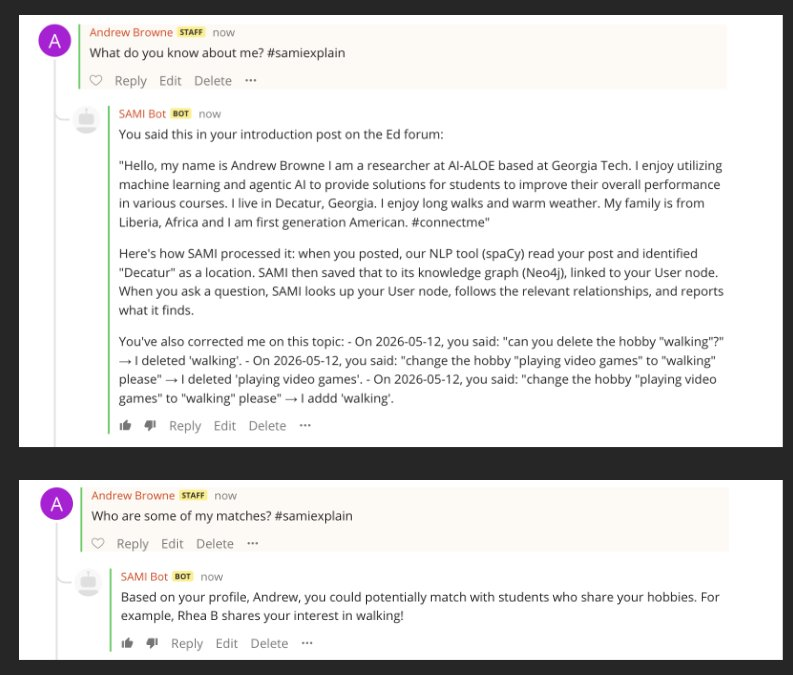
\includegraphics[width=0.85\linewidth]{Figures/sami_samiexplain.png}}
	\caption{Example \texttt{\#samiexplain} interactions. Adding \texttt{\#samiexplain} to the end of a message prompts SAMI to explain the reasoning behind its answer or recommendation.}
	\label{fig:samiexplain}
\end{figure}

\subsection{SAMI's model of you (\#correctme)}

% INSTRUCTIONS (for your reference — not rendered in the PDF):
% Ask SAMI what it knows about you by adding #correctme at the end of your
% message. Is its model of you correct? If not, provide a correction update
% and ask SAMI to revise its knowledge of you. Did it do so correctly?

\todo[inline]{Ask SAMI what it knows about you by adding \#correctme at the end of your message. Report its model of you, then assess: Is it correct? If not, provide a correction update and ask SAMI to revise its knowledge of you. Did it revise correctly?}

% NOTE: The figure below is a provided reference image showing an example
% #correctme interaction. The image file lives in the Figures/ folder.
% It is illustrative — you may keep it for context or delete it; either way,
% replace the orange box above with your own interaction findings.
\begin{figure}[h]
	\centering
	\fbox{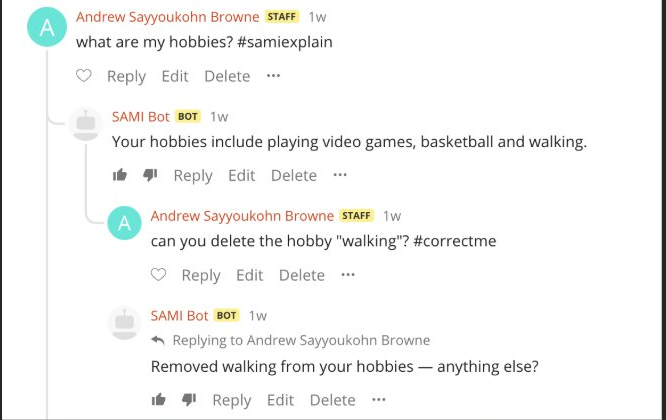
\includegraphics[width=0.8\linewidth]{Figures/sami_correctme.png}}
	\caption{Example \texttt{\#correctme} interaction. Adding \texttt{\#correctme} to the end of a message lets you correct SAMI's model of you (here, removing ``walking'' from the user's hobbies).}
	\label{fig:correctme}
\end{figure}

\subsection{Explanations of revisions}

% INSTRUCTIONS (for your reference — not rendered in the PDF):
% Ask SAMI to explain its revisions to you. Are the explanations useful? Do
% they increase your trust in SAMI?

\todo[inline]{Ask SAMI to explain the revisions it made to its model of you. Report what it said, then assess: Are the explanations useful? Do they increase your trust in SAMI?}

\subsection{Reflection on performance}

% INSTRUCTIONS (for your reference — not rendered in the PDF):
% Write a short reflection on SAMI's performance. What are the biggest
% limitations, shortcomings, or gaps you noticed?

\todo[inline]{Write a short reflection on SAMI's overall performance based on the audit above. What are the biggest limitations, shortcomings, or gaps you noticed? These findings will motivate your redesign in Part 2.}


% #############################################################################
%                   PART 2: THE REDESIGN CHALLENGE
% #############################################################################
\section{The redesign challenge}

% ~~~~~~~~~~~~~~~~~~~~~~~~~~~~~~~~~~~~~~~~~~~~~~~~~~~~~~~~~~~~~~~~~~~~~~~~~~~~~
% INSTRUCTIONS (for your reference — not rendered in the PDF):
%
% Reflect on the limitations you found in Part 1 and propose a feasible
% one-semester improvement plan for ONE OR MORE of these three components:
%
% 1. KNOWLEDGE GRAPH (KG) EXPANSION
%    Reflection: Briefly describe SAMI's knowledge graph. Critique it.
%    Proposal: What new Entity Types or Relationships should be added?
%
% 2. MATCHMAKING LOGIC
%    Reflection: Briefly describe how SAMI connects you with others. Critique it.
%    Proposal: Propose a new process or heuristic.
%
% 3. THE INTERACTION & FEEDBACK LOOP
%    Reflection: Briefly summarize your interactions with SAMI. Critique them
%      from the perspectives of transparency and trust.
%    Proposal: Suggest a new feedback loop (e.g., how should SAMI explain
%      itself to you, and how should SAMI update itself based on your feedback).
%
% Your response is a concise "Product Roadmap" with the four parts below:
% Component Selection, The Critique, The High-Level Vision, The Technical
% Roadmap. Use the reflection/proposal prompts above for whichever
% component(s) you choose.
% ~~~~~~~~~~~~~~~~~~~~~~~~~~~~~~~~~~~~~~~~~~~~~~~~~~~~~~~~~~~~~~~~~~~~~~~~~~~~~

\subsection{Component selection}

% INSTRUCTIONS (for your reference — not rendered in the PDF):
% Which of the three areas will you prioritize? (Knowledge Graph Expansion,
% Matchmaking Logic, or the Interaction & Feedback Loop — one or more.)

\todo[inline]{State which of the three components you will prioritize: Knowledge Graph (KG) Expansion, Matchmaking Logic, or the Interaction \& Feedback Loop (you may choose one or more). Briefly justify your choice based on the limitations you found in Part 1.}

\subsection{The critique}

% INSTRUCTIONS (for your reference — not rendered in the PDF):
% A clear diagnosis of WHY the current version fails in this area. Draw on the
% component-specific reflection prompts:
%   - KG: describe SAMI's knowledge graph and critique it.
%   - Matchmaking: describe how SAMI connects you with others and critique it.
%   - Feedback Loop: summarize your interactions and critique them from the
%     perspectives of transparency and trust.

\todo[inline]{Provide a clear diagnosis of why the current version of SAMI fails in your selected component. For the Knowledge Graph, describe and critique SAMI's knowledge graph. For Matchmaking Logic, describe and critique how SAMI connects you with others. For the Interaction \& Feedback Loop, summarize your interactions and critique them from the perspectives of transparency and trust.}

\subsection{The high-level vision}

% INSTRUCTIONS (for your reference — not rendered in the PDF):
% What does "success" look like for this component by the end of the semester?

\todo[inline]{Describe your high-level vision: What does ``success'' look like for this component by the end of the semester?}

\subsection{The technical roadmap}

% INSTRUCTIONS (for your reference — not rendered in the PDF):
% Provide 3-4 concrete steps you would take to implement this. Include your
% proposal: new Entity Types/Relationships (KG), a new process or heuristic
% (Matchmaking), or a new feedback loop (Interaction & Feedback Loop).
% Example: "Step 1: Scrape LinkedIn API to enrich entity attributes;
%           Step 2: Implement a Vector Database for faster relationship
%           querying..."

\todo[inline]{Provide 3--4 concrete implementation steps for your selected component. Incorporate your specific proposal: new Entity Types or Relationships (Knowledge Graph), a new process or heuristic (Matchmaking Logic), or a new feedback loop describing how SAMI should explain itself and update based on your feedback (Interaction \& Feedback Loop). For example: ``Step 1: Scrape LinkedIn API to enrich entity attributes; Step 2: Implement a Vector Database for faster relationship querying\ldots''}


% #############################################################################
%                             REFERENCES
% #############################################################################
\section{References}
\printbibliography[heading=none]


% #############################################################################
%                APPENDICES (OPTIONAL — NOT GRADED)
% #############################################################################
\section{Appendices (optional --- not graded)}

\textbf{IMPORTANT:} This section is entirely optional. Nothing in the appendices will be used in grading. All graded content must appear in the main body (Parts 1 and 2). Appendices are provided only for optional supplementary material (e.g., interaction transcripts, screenshots, or extended analysis) that may help your classmates and grader give better feedback. If you have no appendices, delete this entire section.

% TIP: Paste any SAMI interaction transcripts inside the
% \begin{transcript} ... \end{transcript} environment below. It automatically
% wraps long lines and needs no special character escaping. To include
% screenshots instead, use the figure example in the formatting section.

% \subsection{SAMI interaction transcripts}
%
% \begin{transcript}
% [Paste your SAMI interaction transcript here.]
% \end{transcript}


% #############################################################################
% JDF FORMATTING EXAMPLES (DELETE BEFORE SUBMISSION)
% #############################################################################

\section*{JDF formatting examples (delete before submission)}

\textit{This section is provided as a reference for JDF formatting conventions.
Delete it entirely before submitting your assignment.}

\subsection*{Figure example}

To include a figure (e.g., a SAMI screenshot or a roadmap diagram), uncomment and adapt the code below:

% \begin{figure}[h]
% 	\centering
% 	\includegraphics[height=6cm]{Figures/your_image.png}
% 	\caption{A descriptive caption of what the figure shows. Source: [citation].}
% 	\label{fig:example_figure}
% \end{figure}

To reference a figure in text: ``As shown in Figure~1\ldots'' (use \verb|\ref{fig:your_label}| once the figure is uncommented).

Figures should always be centered, referenced in text, and include a descriptive caption beneath them. If the figure has a white background, consider adding a $\frac{1}{4}$-point black border for legibility.

\subsection*{Table example}

\begin{table}[h]
	\caption{Example table for a technical roadmap.}
	\small
	\centering
	\begin{tabular}{L{0.12\linewidth} L{0.40\linewidth} L{0.36\linewidth}}
		\textbf{Step} & \textbf{Action} & \textbf{Expected outcome} \\
		\toprule[0.5pt]
		1 & Scrape LinkedIn API to enrich entity attributes & Richer node metadata in the KG \\
		\midrule
		2 & Implement a vector database for relationship querying & Faster, semantic match retrieval \\
		\midrule
		3 & Add a feedback-capture step after each match & Continuous model refinement \\
	\end{tabular}
\end{table}

Table captions go \textit{above} the table (``figures at the foot, tables at the top'').

\subsection*{In-line text formatting}

\textbf{Bold} and \textit{italics} for emphasis. Hyperlinks: \href{https://example.com}{link text}. In-line code: {\tt code here}. Superscripts\textsuperscript{ like this} and subscripts\textsubscript{ like this}.

\subsection*{Quotes}

In-line (fewer than 3 lines): ``Heavy use of peer grading would compromise [the school's] reputation'' (Joyner, 2016).

Block quote (3+ lines):

\begin{quotation}
	\noindent ``Whether or not the grades generated by peers are reliably similar to grades generated by experts is only one factor worth considering, however. Student perception is also an important factor.''
\end{quotation}

\subsection*{Lists}

Bullet points:

\begin{itemize}
	\item First bullet point item
	\item Second bullet point item
\end{itemize}

Numbered list:

\begin{enumerate}
	\item First numbered item
	\item Second numbered item
\end{enumerate}

\subsection*{Citations}

Parenthetical: \verb|\citep{key}|. In-text: \verb|\citeauthor{key} (\citeyear{key})|. Multiple: \verb|(\cite{key1}; \cite{key2})|. Place citations close to the claim, not just at paragraph end.

\subsection*{Footnotes}

In-line citations are preferred over footnotes. If you do use footnotes, they should be 8.5 pt with 14 pt line spacing. Example: \verb|\footnote{Your footnote text here.}|

\subsection*{Reference list}

References are handled by \verb|\printbibliography|. They should be numbered, alphabetical by first author's last name. Same author with multiple papers: chronological order (oldest first). Same author and year: append a letter (e.g., 2018a, 2018b). Only include works cited in-line. The reference list does not count against the page count.

\subsection*{Heading 4 example}

\subsubsubsection{Run-in sidehead}\emph{Heading 4} is a run-in sidehead in bold italics, followed by an em dash, flowing into the paragraph text. Use it as a list style rather than a heading style.

\end{document}